% A space X (blob) together with an open cover X = union of U_alpha, drawn as
% nine overlapping dashed open balls (with their centers marked).
% Source: book/tex/topology/compactness.tex (§ open covers).
\documentclass[border=2mm]{standalone}
\usepackage{amssymb}
\usepackage{tikz}
\begin{document}
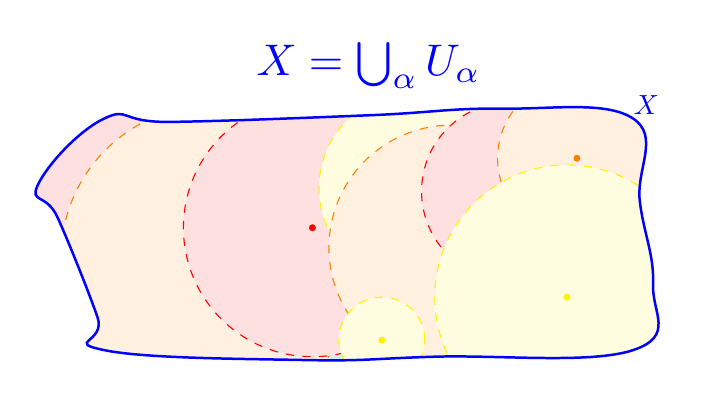
\begin{tikzpicture}[scale=0.42]
  \def\blob{plot[smooth cycle, tension=0.7]
    coordinates {(-8,3) (-10,1) (-9.4,0) (-8.2,-3) (-8,-4) (-2,-4.3)
                 (2,-4.2) (8,-4) (8.6,-2) (8.2,0.5) (8,3) (4,3.3)
                 (0,3.1) (-6,2.9)}}
  \begin{scope}
    \clip \blob;
    \fill[cyan!20] \blob;
    \newcommand{\ball}[3]{\fill[#3!12] (#1) circle (#2);
      \draw[#3, dashed] (#1) circle (#2); \fill[#3] (#1) circle (3pt);}
    \ball{-7,0.8}{3.5}{red}
    \ball{-4.7,-1.2}{4.6}{orange}
    \ball{-1.7,-0.3}{3.9}{red}
    \ball{1.4,0.9}{2.9}{yellow}
    \ball{2.5,-0.9}{3.7}{orange}
    \ball{0.4,-3.7}{1.3}{yellow}
    \ball{4.3,0.8}{2.7}{red}
    \ball{6.3,1.8}{2.4}{orange}
    \ball{6.0,-2.4}{4.0}{yellow}
  \end{scope}
  \draw[blue, line width=0.9pt] \blob;
  \node[blue] at (8.4,3.4) {$X$};
  \node[blue, scale=1.6] at (0,4.6) {$X = \bigcup_\alpha U_\alpha$};
\end{tikzpicture}
\end{document}
